% !TEX encoding = UTF-8
% !TEX TS-program = pdflatex
% !TEX root = ../tesi.tex

%**************************************************************
\chapter{L'applicazione}
\label{cap:applicazione}
%**************************************************************

%\intro{Breve introduzione al capitolo}\\

\section{Introduzione alle grammatiche}
Zucchetti negli ultimi anni ha investito molto nella ricerca di una tecnologia che gli permettesse di interagire con i propri prodotti attraverso comandi vocali ed ora sta realizzando delle regole che consentono di generare un numero di \emph{grammatiche} potenzialmente infinito e capace di comprendere ed elaborare il linguaggio naturale.
Gli assistenti virtuali presenti sul mercato sono basati sul seguente concetto: provare a capire tutto ciò che viene detto dagli utenti anche a costo di commettere degli errori. Questa filosofia è mirata a dare all'utente la sensazione di utilizzare uno strumento in grado di capire e ragionare in qualsiasi momento ed è già utilizzata in larga scala da grandi aziende quali Google, Amazon e Apple. Tuttavia, per le funzionalità della maggior parte dei prodotti Zucchetti, tale principio non è applicabile. Infatti necessitano che, quando una frase viene riconosciuta e compresa, il margine di errore sia nullo. Un classico esempio è il trasferimento di denaro in cui se la comprensione del comando avviene in modo errato c'è il rischio di causa danni contingenti agli utenti. \\
Dunque Zucchetti ha intrapreso una strada diversa sviluppando una tecnologia mirata a alla massima precisione accettando talvolta di non riconoscere i comandi ricevuti. Essa consiste quindi in regole molto semplici ed intuitive da applicare a stringhe di testo e riassunte in quattro azioni principali:
\begin{itemize}
	\item concatenazione di elementi;
	\item scelta tra più elementi;
	\item ripetizione di uno o più elementi;
	\item opzionalità di un elemento.
\end{itemize}
A partire da ciò viene costruita una \emph{\gls{gramg}} che permette di interpretare un insieme finito di frasi che rappresentano il dominio della conversazione che si vuole intrattenere. La difficoltà principale è comprendere esattamente l'insieme delle possibili frasi, trovate con un'analisi probabilistica e statistica sul proprio contesto, che si presume l'utente possa dire, senza includere componenti non pertinenti. \\
Un esempio semplice ma dimostrativo di una \emph{\gls{gramg}} che permette di interpretare alcune frasi di saluto è illustrato nella seguente immagine.

\begin{figure}[htbp]
	\begin{center}
		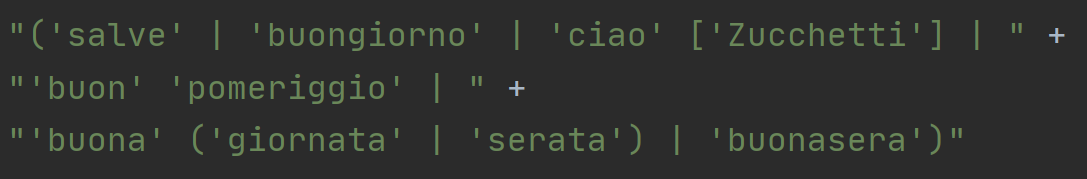
\includegraphics[height=2cm, width=\linewidth]{esempio-grammatica.PNG}
		\caption{Esempio di una grammatica}
	\end{center}
\end{figure}

\vspace{2cm}

Nonostante il loro principio di funzionamento sia relativamente semplice da comprendere, non sono altrettanto facili da interpretare qualora raggiungessero grandi dimensioni e, a maggior ragione, per uno sviluppatore terzo che in futuro le dovrà riutilizzare. Per migliorare questo aspetto l'azienda ha quindi deciso di utilizzare i diagrammi \emph{\gls{rldg}}\glsfirstoccur come strumento di rappresentazione come si può vedere nella figura successiva.

\begin{figure}[htbp]
	\begin{center}
		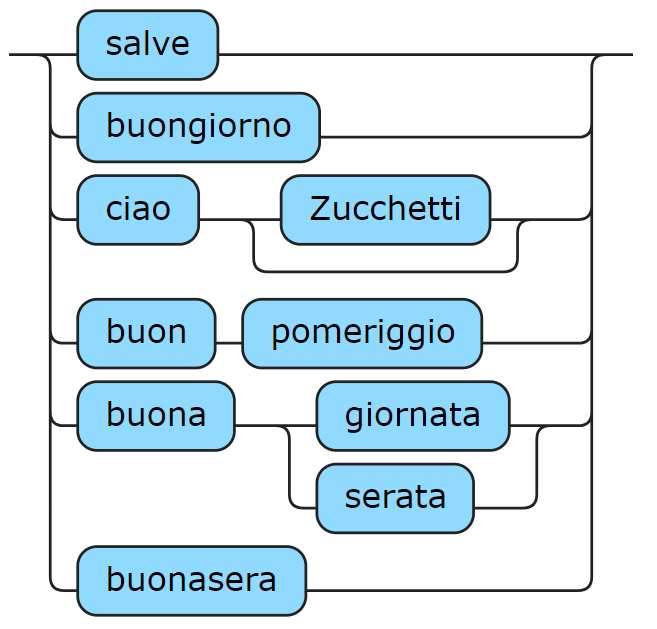
\includegraphics[height=6cm]{esempio-railroad.PNG}
		\caption{Esempio di una grammatica con railroad}
	\end{center}
\end{figure}

Risulta evidente come questa raffigurazione sia molto più efficace e intuitiva. \\
Infine l'applicazione della \emph{\gls{gramg}} sui comandi vocali dell'utente tradotti in stringa avviene attraverso un apposito \emph{\gls{parsg}}\glsfirstoccur sviluppato da Zucchetti che mi è stato consegnato per lo sviluppo del mio progetto.
\section{Analisi dei requisiti}
	\subsection{Descrizione del problema}
	Durante l'attività di ricerca ed analisi svolta sugli assistenti virtuali, in particolare nello sviluppo del \emph{\gls{pocg}} che fa uso di Alexa, è emerso un concetto, caratteristico anche del lavoro che sta svolgendo l'azienda: la conversazionalità. Essa rappresenta la capacità di intrattenere una conversazione da parte di un software simulando quella di una persona. \\
	Inoltre era stato pianificato di costruire una propria \emph{\gls{nlug}} con una \emph{\gls{gramg}} che interpreti un insieme di frasi e dia una risposta ragionata sulla base di esse. \\
	È stato quindi deciso in accordo con il tutor di costruire un'applicazione che metta assieme la realizzazione di una propria \emph{\gls{nlug}} con capacità di conversazione finalizzata al soddisfacimento di una determinata funzionalità, non limitata ad una coppia domanda-risposta. Il dominio è simile a quello del \emph{\gls{pocg}} sviluppato con Alexa ovvero la data di nascita solo che molto più completo. In particolare prevede che le frasi pronunciate dall'utente possano essere composte dai seguenti elementi:
	\begin{itemize}
		\item saluto iniziale opzionale;
		\item un insieme completo di frasi introduttive per esprimere la data di nascita nel formato giorno, mese e anno o, alternativamente, la data di compleanno nel formato giorno, mese;
		\item insieme completo di espressioni per la data di nascita e conseguentemente del sottoinsieme data di compleanno;
		\item insieme di frasi per riconoscere come data il giorno di Natale;
		\item insieme di frasi per riconoscere come data il primo giorno di un qualsiasi mese;
		\item insieme di frasi per interrompere in qualunque momento l'esecuzione;
		\item insieme di frasi per chiedere un eventuale aiuto sulle funzionalità dell'applicazione.
	\end{itemize}
	\subsection{Requisiti}
	Lo scopo principale è dimostrare la fattibilità di costruire una \emph{\gls{nlug}} con la tecnologia sviluppata da Zucchetti che abbia capacità conversazionale. L'applicazione perciò si presenta sotto forma di \emph{\gls{pocg}} e non è quindi integrata in un software aziendale esistente. \\
	Analizzando più in dettaglio gli obiettivi da raggiungere, è stata stilata una lista di requisiti obbligatori la cui fattibilità è certa. Un altro, invece, è emerso ma inserito come opzionale poiché rappresenta un miglioramento ragionevolmente non implementabile nel tempo a disposizione.
	I requisiti obbligatori sono i seguenti:
	\begin{enumerate}
		\item costruzione dell'interfaccia utente:
			\begin{itemize}
				\item interfaccia grafica minimale che permetta all'utente di attivare il riconoscimento del comando vocale;
				\item interfaccia vocale completa di tutti gli accessori studiati durante l'attività di ricerca.
			\end{itemize}
		\item costruzione di una \emph{\gls{nlug}} che comprenda la data di nascita espressa dall'utente, esegua un'elaborazione e prepari di conseguenza una riposta adatta. Deve avere estrema precisione del comprendere le frasi una volta riconosciute anche a costo di rigettarne alcune.
		\item implementazione della capacità conversazionale con memoria al fine di portare a compimento la funzionalità in esecuzione dando maggiormente la percezione all'utente di dialogare con una persona.
	\end{enumerate}
	Il requisito opzionale è il seguente:
	\begin{itemize}
		\item generalizzazione della grammatica in modo che permetta non solo di interpretare l'input dell'utente ma anche di generare la risposta sulla base dell'elaborazione.
	\end{itemize}
\section{Progettazione}
	\subsection{Interfaccia vocale}
	\subsection{NLU}
	\subsection{Capacità conversazionale}

\section{Implementazione}

\section{Test}

\section{Sviluppi futuri}
